% file: chap6.tex

\chapter{深度学习}
\label{ch:Deeplearning}

在\hyperref[ch:WhyHardToTrain]{上一章},我们学习了深度神经网络通常比浅层神经网络
更加难以训练。我们有理由相信,若是可以训练深度网络,则能够获得比浅层网络更加强大
的能力,但是现实很残酷。从上一章我们可以看到很多不利的消息,但是这些困难不能阻止
我们使用深度神经网络。本章,我们将给出可以用来训练深度神经网络的技术,并在实战中
应用它们。同样我们也会从更加广阔的视角来看神经网络,简要地回顾近期有关深度神经网
络在图像识别、语音识别和其他应用中的研究进展。然后,还会给出一些关于未来神经网络
又或人工智能的简短的推测性的看法。

这一章比较长。为了更好地让你们学习,我们先粗看一下整体安排。本章的小结之间关联并
不太紧密,所以如果读者熟悉基本的神经网络的知识,那么可以任意跳到自己最感兴趣的部
分。

\hyperref[sec:convolutional_networks]{本章主要的部分}是对最为流行神经网络之一的深
度卷积网络的介绍。我们将细致地分析一个使用卷积网络来解决 MNIST 数据集的手写数字识
别的例子(包含了代码和讲解):
\begin{center}
  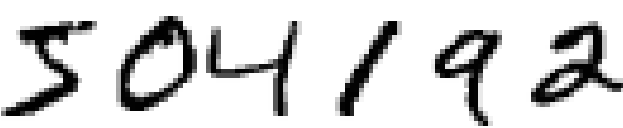
\includegraphics[width=64pt]{digits}
\end{center}

我们将从浅层的神经网络开始来解决上面的问题。通过多次的迭代,我们会构建越来越强大
的网络。在这个过程中,也将要探究若干强大技术:卷积、pooling、使用GPU来更好地训练、
训练数据的算法性扩展(避免过匹配)、dropout 技术的使用(同样为了防止过匹配现象)、
网络的 ensemble 使用 和 其他技术。最终的结果能够接近人类的表现。
在 10,000 幅 MNIST 测试图像上 —— 模型从未在训练中接触的图像 —— 该系统最终能够将其
中 9,967 幅正确分类。这儿我们看看错分的 33 幅图像。注意正确分类是右上的标记;系统
产生的分类在右下:
\begin{center}
  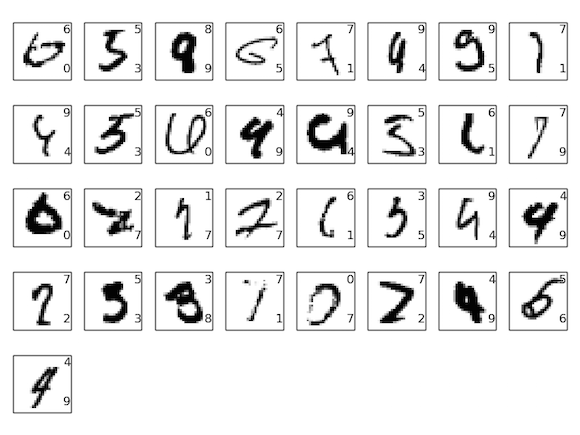
\includegraphics[width=.75\textwidth]{ensemble_errors}
\end{center}

可以发现,这里面的图像对于正常人类来说都是非常困难区分的。例如,在第一行的第三幅
图。我看的话,看起来更像是 “9” 而非 “8”,而 “8” 却是给出的真实的结果。我们
的网络同样能够确定这个是 “9”。这种类型的“错误” 最起码是容易理解的,可能甚至值
得我们赞许。最后用对最近使用深度(卷积)神经网络在图像识别上的研究进展作为关于图
像识别的讨论的总结。

本章剩下的部分,我们将会从一个更加宽泛和宏观的角度来讨论深度学习。概述一些神经网
络的其他模型,例如 RNN 和 LSTM 网络,以及这些网络如何在语音识别、自然语言处理和其
他领域中应用的。最后会试着推测一下,神经网络和深度学习未来发展的方向,会
从 intention-driven user interfaces 谈谈深度学习在人工智能的角色。这章内容建立在
本书前面章节的基础之上,使用了前面介绍的诸如 BP、规范化、softmax 函数,等等。然而,
要想阅读这一章,倒是不需要太过细致地掌握前面章节中内容的所有的细节。当然读完第一
章关于神经网络的基础是非常有帮助的。本章提到第二章到第五章的概念时,也会在文中给
出链接供读者去查看这些必需的概念。

需要注意的一点是,本章所没有包含的那一部分。这一章并不是关于最新和最强大的神经网
络库。我们也不是想训练数十层的神经网络来处理最前沿的问题。而是希望能够让读者理解
深度神经网络背后核心的原理,并将这些原理用在一个 MNIST 问题的解决中,方便我们的理
解。换句话说,本章目标不是将最前沿的神经网络展示给你看。包括前面的章节,我们都是
聚焦在基础上,这样读者就能够做好充分的准备来掌握众多的不断涌现的深度学习领域最新
工作。本章仍然在Beta版。期望读者指出笔误,bug,小错和主要的误解。如果你发现了可疑
的地方,请直接联系 mn@michaelnielsen.org。

\section{介绍卷积网络}
\label{sec:convolutional_networks}

在前面的章节中,我们教会了神经网络能够较好地识别手写数字:
\begin{center}
  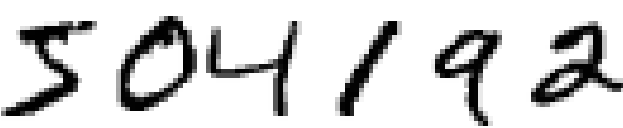
\includegraphics[width=64pt]{digits}
\end{center}

我们在深度神经网络中使用全连接的邻接关系。网络中的神经元与相邻的层上的所有神经元
均连接:
\begin{center}
  \includegraphics{tikz41}
\end{center}

特别地,对输入图像中的每个像素点,我们将其光强度作为对应输入层神经元的输入。对
于 $28 \times 28$ 像素的图像,这意味着我们我们的网络需要有
$784$($= 28 \times 28$)个输入神经元。我们然后训练网络的权重和偏差,使得网络输出
能够 —— 如我们希望地 —— 正确地辨认输入图像:'0', '1', '2', ..., '8', or '9'。

我们之前地网络工作得相当好:...

卷积神经网络采用了三种基本概念:\emph{局部感受野\index{局部感受野}(local
  receptive fields\index{local receptive fields)},\emph{共享权重\index{共享权
      重}(shared weights\index{shared weights})},和\emph{混合储存\index{混合储
      存}(pooling\index{pooling})}。让我们逐个看下:

\textbf{局部感受野:} 

\begin{center}
  \includegraphics{tikz42}
\end{center}

\begin{center}
  \includegraphics{tikz43}
\end{center}

\begin{center}
  \includegraphics{tikz44}
\end{center}

\begin{center}
  \includegraphics{tikz45}
\end{center}

\textbf{共享权重和偏差:}

\begin{equation}
  \sigma\left(b + \sum_{l=0}^4 \sum_{m=0}^4  w_{l,m} a_{j+l, k+m} \right)
  \label{eq:125}\tag{125}
\end{equation}

\begin{center}
  \includegraphics{tikz46}
\end{center}

\textbf{混合储存层:}

\begin{center}
  \includegraphics{tikz47}
\end{center}

\textbf{综合在一起:}

\subsection*{问题}

\begin{itemize}
  \item \textbf{卷积网络中的反向传播}\quad 
\end{itemize}

\section{卷积神经网络在实际中的应用}
\label{seq:convolutional_neural_networks_in_practice}

\begin{lstlisting}[language=Python]
>>> import network3
>>> from network3 import Network
>>> from network3 import ConvPoolLayer, FullyConnectedLayer, SoftmaxLayer
>>> training_data, validation_data, test_data = network3.load_data_shared()
>>> mini_batch_size = 10
>>> net = Network([
        FullyConnectedLayer(n_in=784, n_out=100),
        SoftmaxLayer(n_in=100, n_out=10)], mini_batch_size)
>>> net.SGD(training_data, 60, mini_batch_size, 0.1, 
            validation_data, test_data)
\end{lstlisting}

\section{卷积网络的代码}
\label{sec:the_code_for_our_convolutional_networks}

\section{图像识别领域中的近期进展}
\label{sec:recent_progress_in_image_recognition}

\section{其他的深度学习模型}
\label{sec:other_approaches_to_deep_neural_nets}

\section{神经网络的未来}
\label{sec:on_the_future_of_neural_networks}
